% TODO: Zeit für Arbeit, Arbeit für Zeit
\chapter{Die Zeit zu bestimmen erfordert Arbeit}
\label{les:17}

\begin{chapquote}{Lewis Carroll, \textit{Alice im Wunderland}}
\enquote{Ach herrje! Ich werde zu spät kommen!}
\end{chapquote}

Es wird oft gesagt, dass Bitcoins \enquote{geschürft} werden weil tausende von
Computern an der Lösung \textit{sehr komplexer} mathematischer Probleme
arbeiten. Probleme wollen gelöst werden, und wenn man die richtige Antwort
berechnet hat, \enquote{produziert} man einen Bitcoin. Diese vereinfachte
Ansicht des Bitcoin-Minings ist zwar leichter zu verstehen, verfehlt aber den
Sinn etwas. Bitcoins werden nicht produziert oder erschaffen - und es geht nicht
darum mathematische Probleme zu lösen (zudem sind die Probleme nicht
mathematisch komplex). Es geht darum ein anderes Problem zu lösen: die
\textit{Bestimmung der Zeit} in einem dezentralen System.

Wie im Whitepaper beschrieben ist das Proof-of-Work-System (auch bekannt als
Mining) eine Möglichkeit einen verteilten Zeitstempelserver zu implementieren.

\begin{figure}
  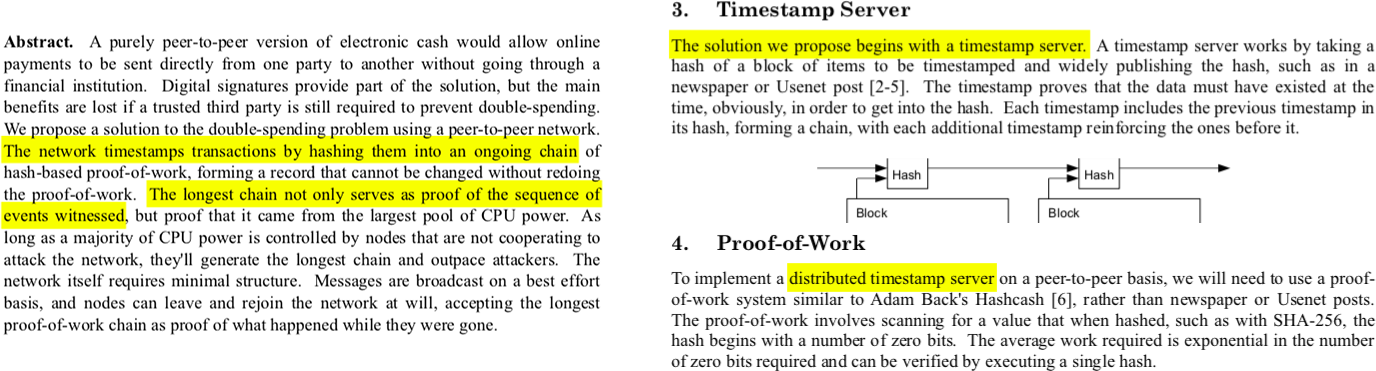
\includegraphics{assets/images/bitcoin-whitepaper-timestamp-wide.png}
  \caption{Excerpts from the whitepaper. Did someone say timechain?}
  \label{fig:bitcoin-whitepaper-timestamp-wide}
\end{figure}

Als ich lernte wie Bitcoin funktioniert dachte auch ich dass Proof-of-Work
ineffizient und verschwenderisch sei. Nach einer Weile begann ich jedoch meine
Sichtweise auf den Energieverbrauch von Bitcoin zu ändern~\cite{gigi:energy}. Es
scheint, dass Proof-of-Work auch heute noch im Jahr 10 n.B. (nach Bitcoin),
weitestgehend missverstanden wird.

Da die Probleme, die beim Proof-of-Work zu lösen sind, frei erfunden werden
glauben viele Menschen, dass es \textit{sinnlose} Arbeit ist. Wenn der Fokus nur
auf der Berechnung liegt, ist dies eine verständliche Schlussfolgerung. Aber bei
Bitcoin geht es nicht um die Berechnung. Es geht darum sich \textit{unabhängig
über die Ordnung der Dinge zu einigen}.

Proof-of-Work ist ein System in dem jeder überprüfen kann was passiert ist und
in welcher Reihenfolge es passiert ist. Diese unabhängige Validierung führt zu
einem Konsens, zu einer individuellen Vereinbarung mehrerer Parteien darüber,
wer was besitzt.

In einer radikal dezentralen Umgebung haben wir nicht den Luxus einer absoluten
Zeit. Jede Uhr würde eine dritte Partei einführen, der man vertrauen müsste,
einen zentralen Punkt im System auf den man sich verlassen muss und der
angegriffen werden kann. \enquote{Das Timing ist das eigentliche Problem}, wie
Grisha Trubetskoy betont~\cite{pow-clock}. Und Satoshi hat dieses Problem durch
die Implementierung einer dezentralen Uhr über eine Proof-of-Work-Blockchain
hervorragend gelöst. Alle sind sich im Voraus einig, dass die Kette mit der
größten kumulierten Arbeit die Quelle der Wahrheit ist. Es ist per Definition
das was tatsächlich passiert ist. Dieses Abkommen ist das was heute als
Nakamoto-Konsens bezeichnet wird.

\begin{quotation}\begin{samepage}
\enquote{Die Netzwerk-Zeitstempel kennzeichnen Transaktionen, indem sie in eine
fortlaufende Kette eingeordnet werden die als Beweis für die Abfolge der
beobachteten Ereignisse dient.}
\begin{flushright} -- Satoshi Nakamoto\footnote{Satoshi Nakamoto, Bitcoin Whitepaper~\cite{whitepaper}}
\end{flushright}\end{samepage}\end{quotation}

Ohne einen konsistenten Weg die Zeit zu definieren kann man kein
\enquote{vorher} und \enquote{nacher} definieren. Eine zuverlässige Ordnung ist
unmöglich. Wie bereits oben erwähnt, ist der Nakamoto-Konsens der Weg Bitcoins
die Zeit konsequent zu bestimmen. Die Anreizstruktur des Systems erzeugt eine
wahrscheinlichkeitsbezogene und dezentrale Uhr, indem sie sowohl die Gier als
auch das Eigeninteresse konkurrierender Teilnehmer nutzt. Die Tatsache, dass
diese Uhr ungenau ist, ist irrelevant da die Reihenfolge der Ereignisse
eindeutig ist und von jedem überprüft werden kann.

Dank des Proof-of-Work sind sowohl die Arbeit als auch die Validierung der
Arbeit radikal dezentralisiert. Jeder kann dem Netzwerk nach Belieben beitreten,
jeder kann das Netzwerk nach Belieben verlassen, und jeder kann alles jederzeit
überprüfen. Nicht nur das, jeder kann den Zustand des Systems
\textit{individuell} überprüfen ohne sich auf andere verlassen zu müssen.

Proof-of-Work zu verstehen erfordert Zeit. Es ist oft kontraintuitiv und obwohl
die Regeln einfach sind führen sie zu recht komplexen Phänomenen. Mir hat es
geholfen meine Sichtweise auf das Mining zu ändern. Nützlich, nicht nutzlos.
Validierung, nicht Berechnung. Zeit, nicht Blöcke.

\paragraph{Bitcoin lehrte mich, dass es schwierig ist die Zeit zu bestimmen,
besonders in dezentralen Systemen.}

% ---
%
% #### Through the Looking-Glass
%
% - [Bitcoin's Energy Consumption: A shift in perspective][energy]
%
% #### Down the Rabbit Hole
%
% - [Blockchain Proof-of-Work Is a Decentralized Clock][points out] by Gregory Trubetskoy
% - [The Anatomy of Proof-of-Work][pow-anatomy] by Hugo Nguyen
% - [PoW is efficient][pow-efficient] by Dan Held
% - [Mining][bw-mining], [Controlled supply][bw-supply] on the Bitcoin Wiki
%
% [points out]: https://grisha.org/blog/2018/01/23/explaining-proof-of-work/
% [energy]: 
% [whitepaper]: https://bitcoin.org/bitcoin.pdf
%
% [pow-efficient]: https://blog.picks.co/pow-is-efficient-aa3d442754d3
% [pow-anatomy]: https://bitcointechtalk.com/the-anatomy-of-proof-of-work-98c85b6f6667
% [bw-mining]: https://en.bitcoin.it/wiki/Mining
% [bw-supply]: https://en.bitcoin.it/wiki/Controlled_supply
%
% <!-- Wikipedia -->
% [alice]: https://en.wikipedia.org/wiki/Alice%27s_Adventures_in_Wonderland
% [carroll]: https://en.wikipedia.org/wiki/Lewis_Carroll
